\documentclass[../main.tex]{subfiles}
\graphicspath{{\subfix{../img/}}}

\begin{document}

\newpage
\section{Hardware Test}
\label{sec:Hardware_Test}
\subsection{Distanz Hindernis}
Um die Bewältigung des Hindernisses erfolgreich durchzuführen, muss die exakte Entfernung zum Hindernis bestimmt werden. Ziel ist es, das Hindernis präzise zwischen den Klemmbacken zu positionieren, ohne dabei mit ihm zu kollidieren. Hierfür stehen zwei bewährte Methoden zur Distanzmessung zur Verfügung: die Messung mittels Schallwellen und die Messung mittels Lichtwellen. In den folgenden Unterkapiteln werden diese Verfahren näher untersucht und getestet.
\subsubsection{Ultraschallsensor}
Für die Messung wird der Ultraschallsensor HC-SR04 verwendet. Dieser Sensor hat eine Reichweite von 2 cm bis 300 cm\footnotemark und arbeitet mit einer Genauigkeit von ±3 mm. Der Sensor wird mit einer Betriebsspannung von 5 V versorgt. Die Messung wird über den Trigger-Pin gestartet, während der Echo-Pin das vom Trigger ausgesendete Signal nach dessen Rückkehr empfängt. Der Zeitunterschied zwischen dem Senden und Empfangen des Signals wird mithilfe der Schallgeschwindigkeit in die Entfernung umgerechnet. Die Genauigkeit des Sensors wird mithilfe des in Abbildung \ref{fig:Ultraschall1} dargestellten Messaufbaus überprüft.
\footnotetext{Quelle: \url{https://www.mikrocontroller.net/attachment/218122/HC-SR04_ultraschallmodul_beschreibung_3.pdf}}

\begin{figure}[h] % 'h' steht für here, was bedeutet, dass das Bild möglichst an dieser Stelle eingefügt wird
    \centering
    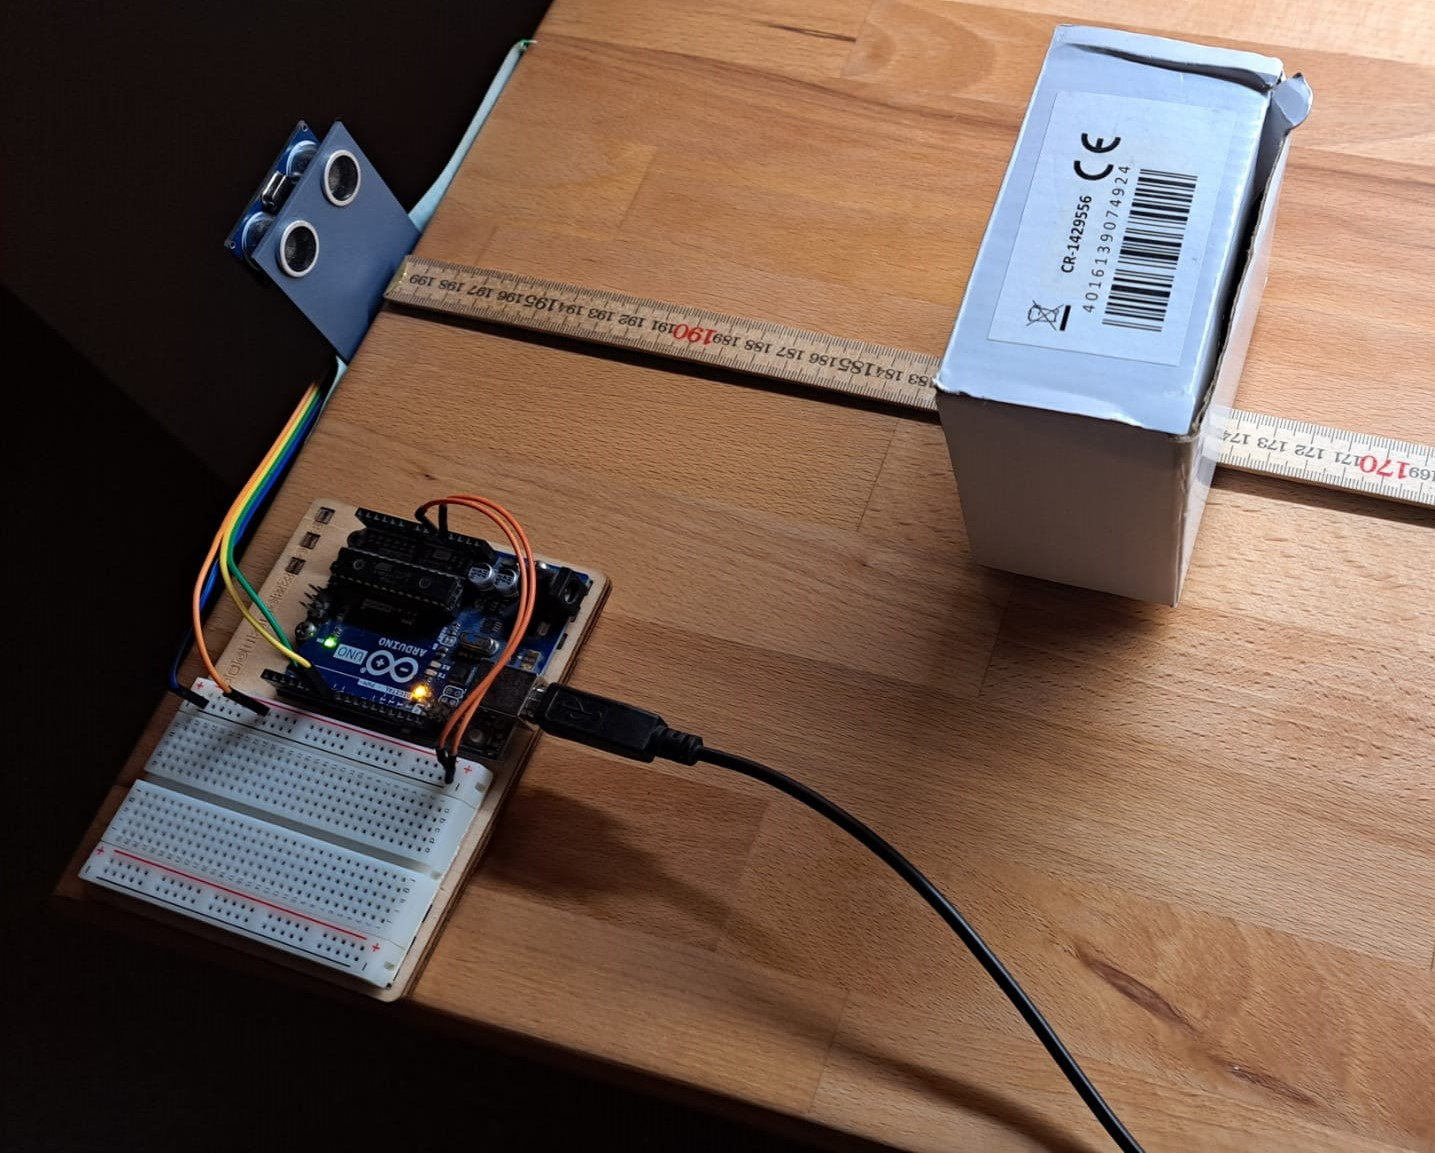
\includegraphics[width=0.5\textwidth]{img/sensortest/MA_Ultraschall.jpg} % Bildname und Breite der Grafik angeben
    \caption{Messaufbau Ultraschallsensor}
    \label{fig:Ultraschall1} % Label für die Referenzierung der Abbildung
\end{figure}

In diesem Messaufbau wird das Objekt schrittweise um jeweils einen Zentimeter verschoben, und der dazugehörige Messwert wird notiert. Die so gewonnenen Daten ergeben die folgenden Messwerte:
\begin{table}[H]
\centering
\begin{minipage}{0.45\textwidth}
\centering
\begin{tabular}{@{}ll@{}}
\toprule
\textbf{Position} & \textbf{Messwert} \\
\midrule
10 mm  & 22 mm  \\
20 mm  & 25 mm  \\
30 mm  & 31 mm  \\
40 mm  & 41 mm  \\
50 mm  & 54 mm  \\
60 mm  & 61 mm  \\
70 mm  & 69 mm  \\
80 mm  & 82 mm  \\
90 mm  & 89 mm  \\
100 mm & 95 mm  \\
\bottomrule
\end{tabular}
\end{minipage}%
\hspace{0.05\textwidth} % kleiner Abstand zwischen den Tabellen
\begin{minipage}{0.45\textwidth}
\centering
\begin{tabular}{@{}ll@{}}
\toprule
\textbf{Position} & \textbf{Messwert} \\
\midrule
110 mm & 112 mm \\
120 mm & 121 mm \\
130 mm & 130 mm \\
140 mm & 136 mm \\
150 mm & 149 mm \\
160 mm & 160 mm \\
170 mm & 170 mm \\
180 mm & 181 mm \\
190 mm & 190 mm \\
200 mm & 205 mm \\
\bottomrule
\end{tabular}
\end{minipage}
\caption{Ultraschallsensor Messwerte}
\label{tab:UltraschallMD}
\end{table}

Aus der in Tabelle \ref{tab:UltraschallMD} dargestellten Messwerte wird ersichtlich, dass die Genauigkeit des Sensors in unmittelbarer Nähe zum Objekt geringer ist. Mit zunehmendem Abstand des Objekts verbessert sich die Präzision der Messungen. Dies bedeutet, dass der Ultraschallsensor so positioniert werden sollte, dass sich sein Einbauort mindestens 3 cm vom Hindernis entfernt befindet.

\newpage
\subsubsection{Time of Flight Sensor}
Ein Time-of-Flight-Sensor (TOF) arbeitet nach einem ähnlichen Prinzip wie ein Ultraschallsensor, jedoch sendet er statt Schallwellen einen Lichtstrahl aus. In diesem Experiment wird der TOF-Sensor vom Typ VL530L0X getestet. Der Messaufbau entspricht dem des Ultraschallsensors (siehe Abbildung \ref{fig:TOF1}). Die Kommunikationsart lauft über den I2C Bus.

\begin{figure}[h!] % 'h' steht für here, was bedeutet, dass das Bild möglichst an dieser Stelle eingefügt wird
    \centering
    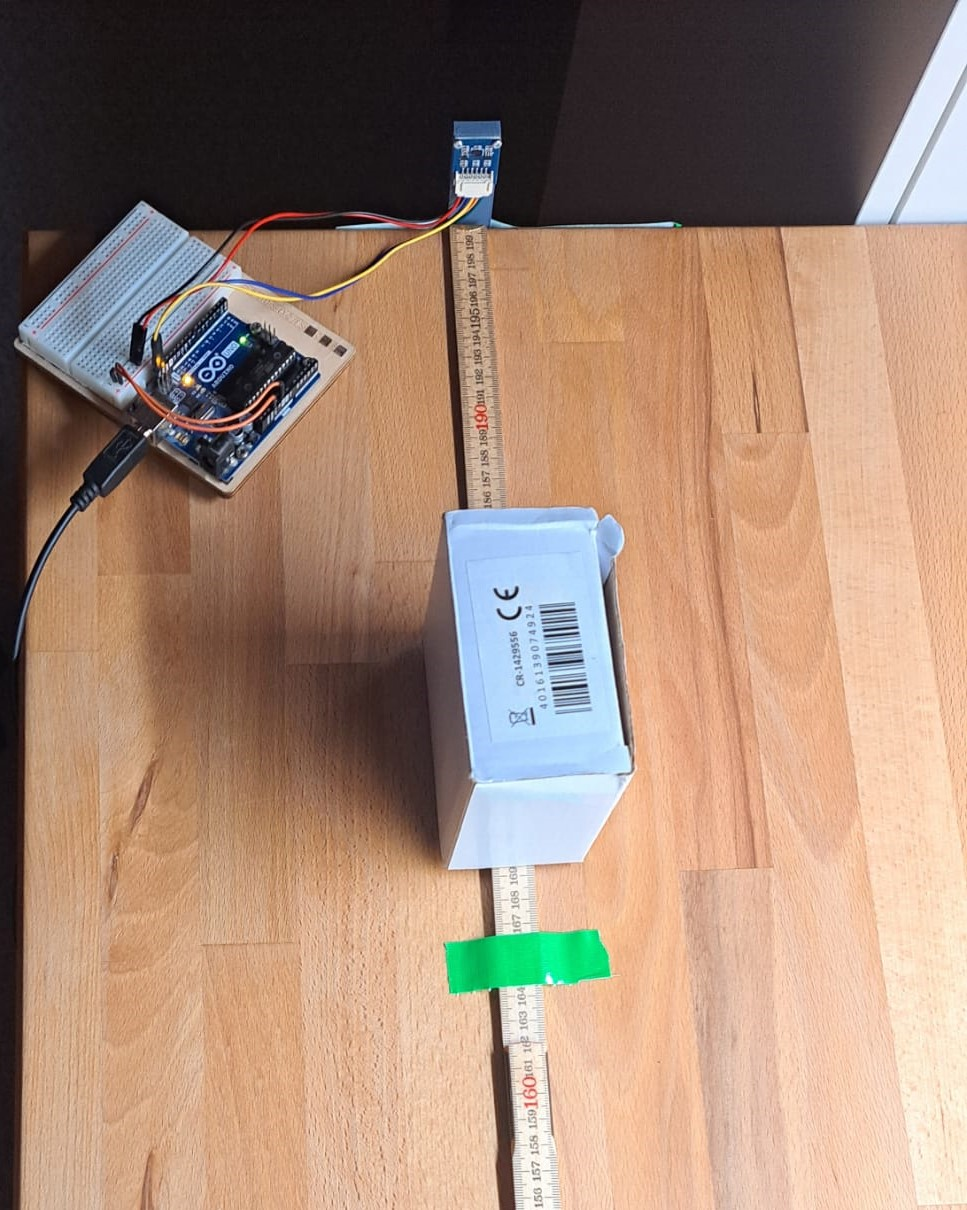
\includegraphics[width=0.35\textwidth]{img/sensortest/MA_TOF.jpg} % Bildname und Breite der Grafik angeben
    \caption{Testaufbau TOF Sensor}
    \label{fig:TOF1} % Label für die Referenzierung der Abbildung
\end{figure}


Auch bei diesem Experiment wird das Objekt schrittweise um jeweils einen Zentimeter nach vorne bewegt, und die entsprechenden Messdaten werden aufgezeichnet. Die dabei ermittelten Werte sind wie folgt:
\begin{table}[H]
\centering
\begin{minipage}{0.45\textwidth}
\centering
\begin{tabular}{@{}ll@{}}
\toprule
\textbf{Position} & \textbf{Messwert} \\
\midrule
10 mm  & 11 mm  \\
20 mm  & 24 mm  \\
30 mm  & 31 mm  \\
40 mm  & 43 mm  \\
50 mm  & 51 mm  \\
60 mm  & 63 mm  \\
70 mm  & 72 mm  \\
80 mm  & 84 mm  \\
90 mm  & 93 mm  \\
100 mm & 102 mm \\
\bottomrule
\end{tabular}
\end{minipage}%
\hspace{0.05\textwidth} % kleiner Abstand zwischen den Tabellen
\begin{minipage}{0.45\textwidth}
\centering
\begin{tabular}{@{}ll@{}}
\toprule
\textbf{Position} & \textbf{Messwert} \\
\midrule
110 mm & 115 mm \\
120 mm & 125 mm \\
130 mm & 132 mm \\
140 mm & 145 mm \\
150 mm & 151 mm \\
160 mm & 163 mm \\
170 mm & 170 mm \\
180 mm & 182 mm \\
190 mm & 190 mm \\
200 mm & 200 mm \\
\bottomrule
\end{tabular}
\end{minipage}
\caption{TOF Messwerte}
\label{tab:TOFMD}
\end{table}

Aus der Tabelle \ref{tab:TOFMD} wird ersichtlich, dass die Messwerte des TOF-Sensors in der Nähe des Sensors bessere Messungen liefert. Ebenso liefert der Sensor zuverlässige Ergebnisse in grösserer Entfernung. Jedoch ändert sich dies schnell bei Sonnenlicht Einstrahlung. In diesem Fall sind die Werte sehr inkonsistent. Daher wird der Ultraschallsensor als zuverlässiger eingeschätzt.

\subsection{Linienerkennung / Punkterkennung}
\subsubsection{Farbsensor}
Der in diesem Experiment getestete Farbsensor trägt die Typenbezeichnung TCS34725. Er kommuniziert über eine I2C-Schnittstelle und liefert Messwerte für Rot-, Grün- und Blauanteile sowie den Clear-Wert. Darüber hinaus können aus diesen Werten der Farbtemperatur- und der Lux-Wert berechnet werden. Ziel dieses Tests ist es, den Wert zu ermitteln, der auf unterschiedlichen Bodeneigenschaften die grössten Unterschiede zeigt. Um reproduzierbare Messungen zu gewährleisten, wurde ein spezieller Halter angefertigt, der den Sensor in einer konstanten Höhe von 1 cm über dem Boden positioniert (siehe Abbildung \ref{fig:Farbsensorhalter}).

\begin{figure}[H] % 'h' steht für here, was bedeutet, dass das Bild möglichst an dieser Stelle eingefügt wird
    \centering
    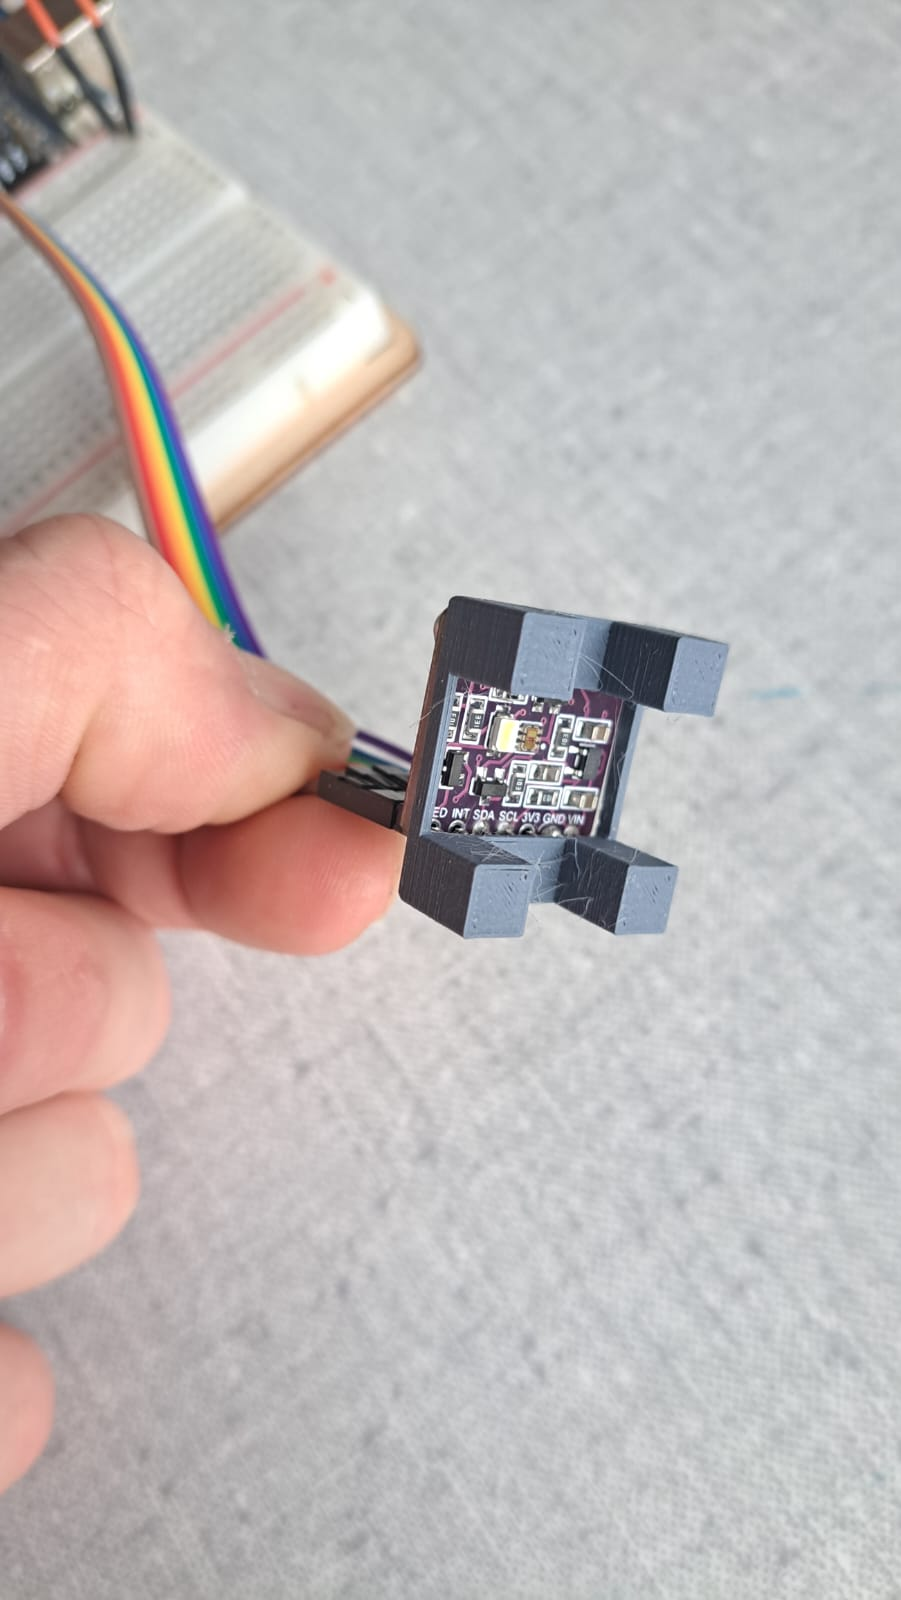
\includegraphics[width=0.2\textwidth]{img/sensortest/FarbsensorHalter.jpg} % Bildname und Breite der Grafik angeben
    \caption{Farbsensorhalter}
    \label{fig:Farbsensorhalter} % Label für die Referenzierung der Abbildung
\end{figure}

Im nächsten Schritt werden alle vier möglichen Szenarien getestet, wie in Abbildung \ref{fig:Testanordnungen} dargestellt. Dabei handelt es sich um folgende Fälle: die Linie, den weissen Punkt, die rote Platte und die Fuge. Während aller Tests bleibt die LED des Sensors dauerhaft eingeschaltet, um konsistente Beleuchtungsbedingungen zu gewährleisten.

\begin{figure}[H]
    \centering
    % Oben links
    \begin{subfigure}{0.3\textwidth} % Breite auf 45% gesetzt, um Platz für zwei Bilder pro Zeile zu schaffen
        \centering
        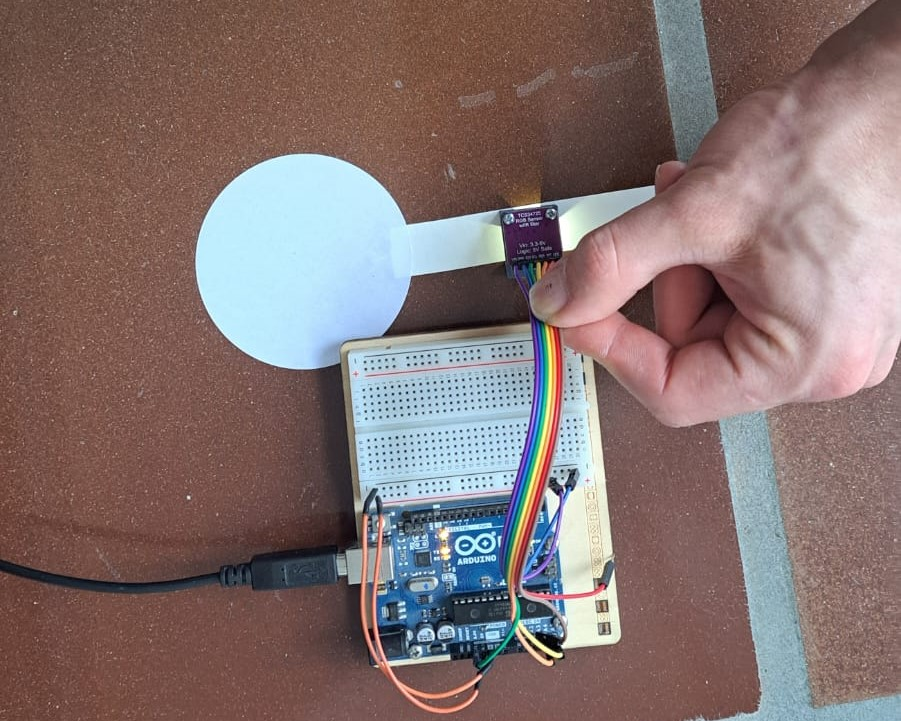
\includegraphics[width=\linewidth]{img/sensortest/Farbsensor_Linie.jpg}
        \caption{Farbsensor Linie}
        \label{fig:FarbsensorLinie}
    \end{subfigure}
    % Oben rechts
    \begin{subfigure}{0.3\textwidth}
        \centering
        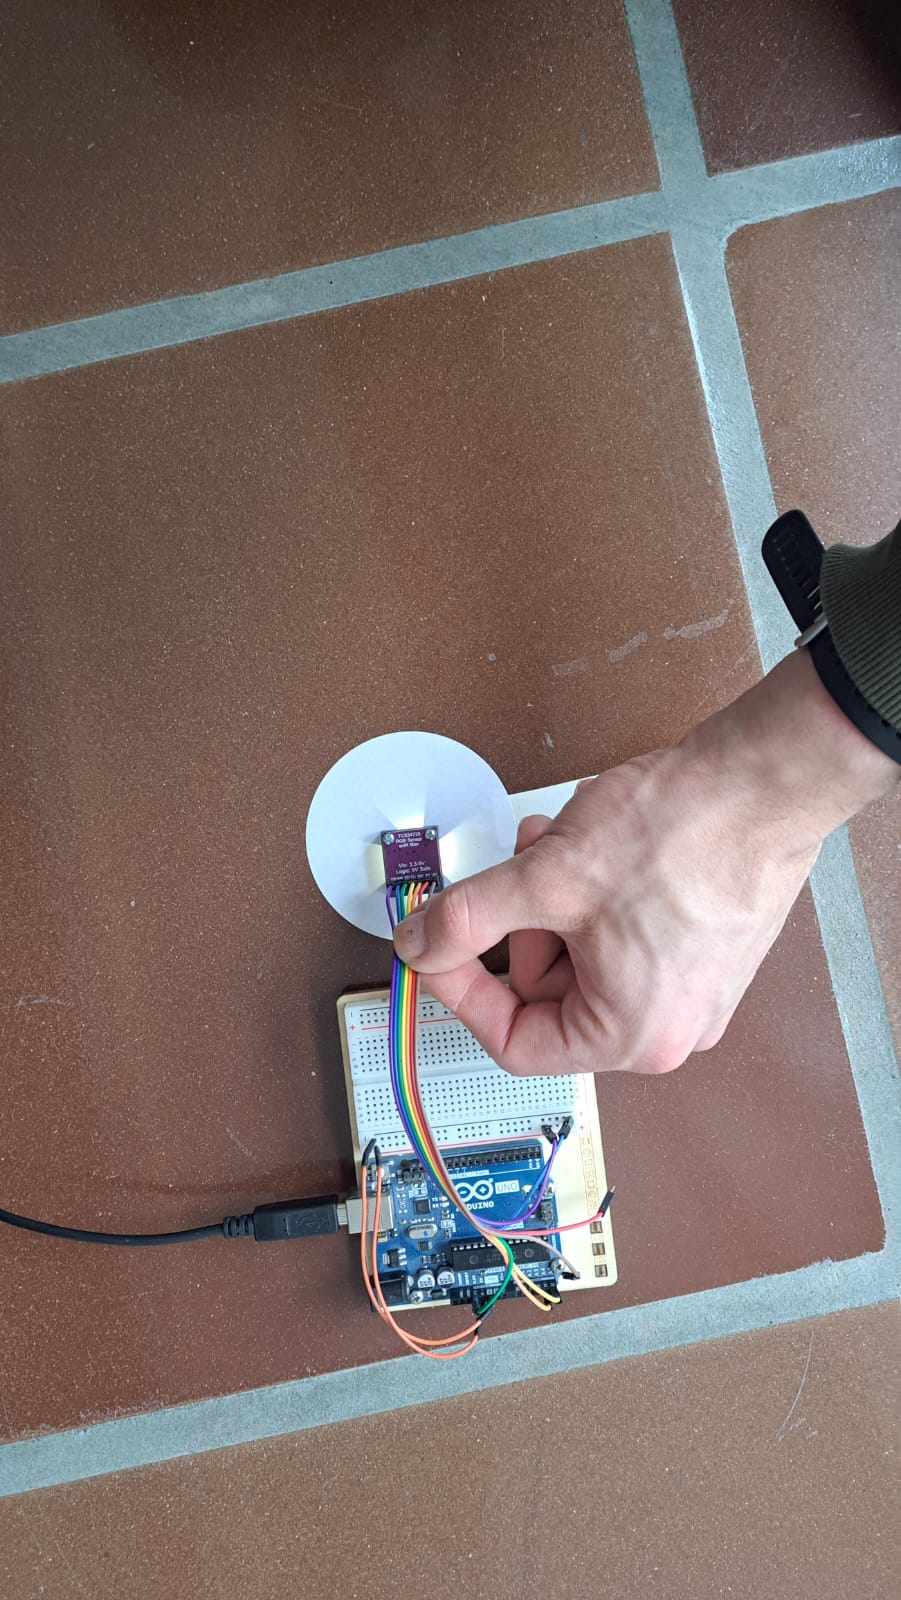
\includegraphics[width=\linewidth]{img/sensortest/Farbsensor_WeisserPunkt.jpg}
        \caption{Farbsensor weisser Punkt}
        \label{fig:FarbsensorWeisserPunkt}
    \end{subfigure}
    
    % Abstand zwischen den Reihen
    \vspace{0.5cm}

    % Unten links
    \begin{subfigure}{0.3\textwidth}
        \centering
        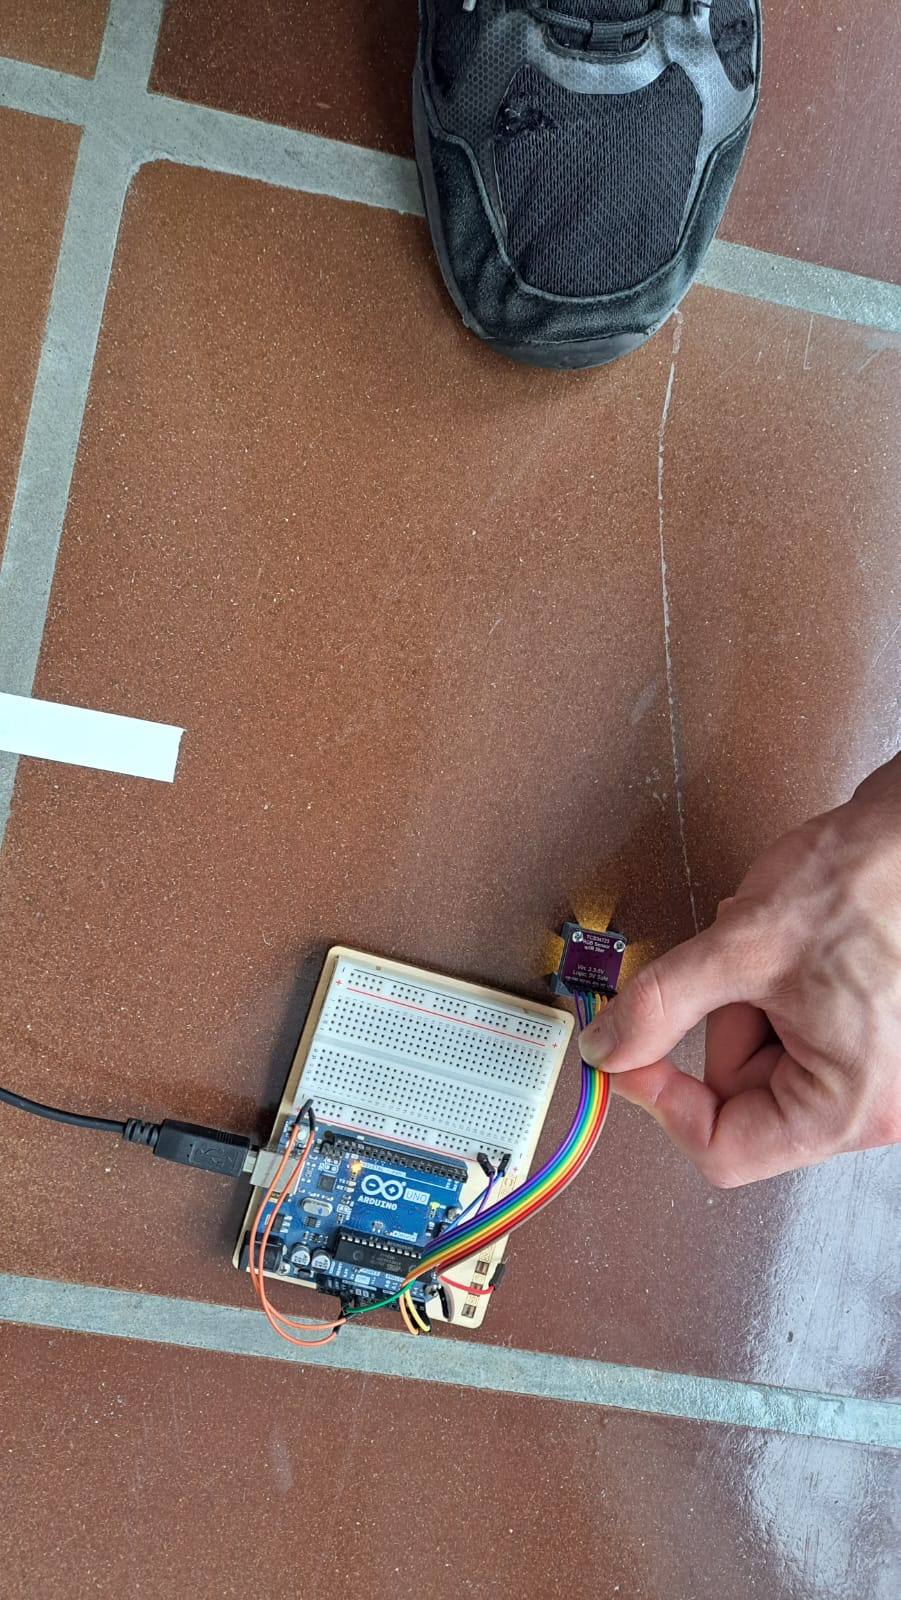
\includegraphics[width=\linewidth]{img/sensortest/Farbsensor_Platte.jpg}
        \caption{Farbsensor Platte}
        \label{fig:FarbsensorPlatte}
    \end{subfigure}
    % Unten rechts
    \begin{subfigure}{0.3\textwidth}
        \centering
        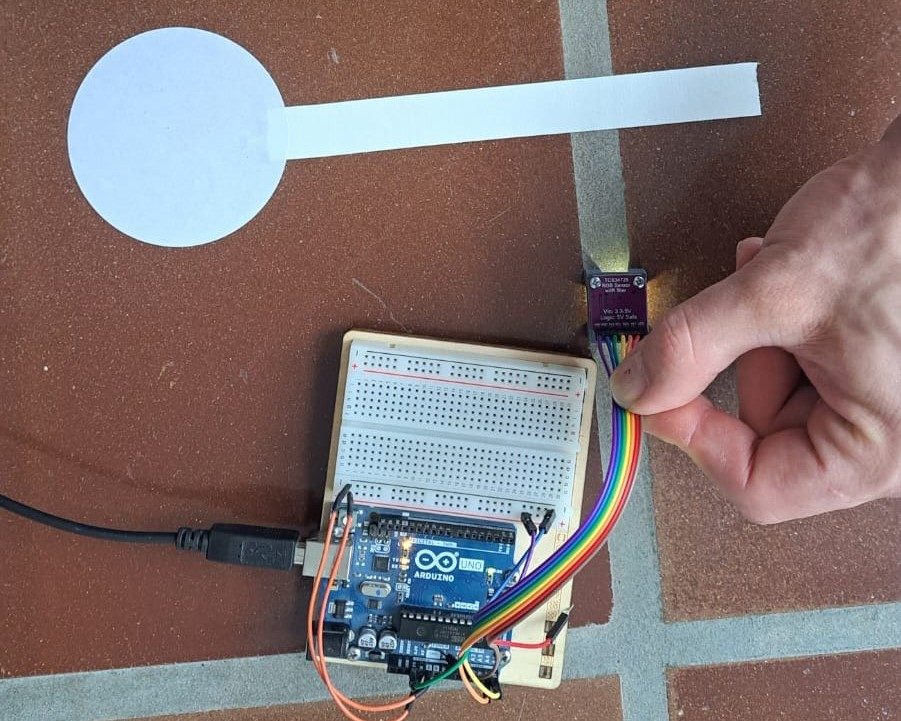
\includegraphics[width=\linewidth]{img/sensortest/Farbsensor_Fuge.jpg}
        \caption{Farbsensor Fuge}
        \label{fig:FarbsensorFuge}
    \end{subfigure}

    \caption{Testaufbau}
    \label{fig:Testanordnungen}
\end{figure}


Der Farbsensor kann über die I2C-Schnittstelle konfiguriert werden, wobei unter anderem die Belichtungszeit angepasst werden kann. In diesem Test wurde die Belichtungszeit auf 101 ms eingestellt, um den Kontrast zwischen den Bodenelementen zu erhöhen. Es hat sich gezeigt, dass mit einer längeren Belichtungszeit die Differenz zwischen den verschiedenen Bodenelementen grösser wird. Allerdings waren die Differenzen bei einer Belichtungszeit von weniger als 101 ms zu gering, um eine signifikante Unterscheidung zu ermöglichen.

Die durchgeführten Tests lieferten die folgenden Messdaten:


\begin{figure}[H]
    \centering
    % Oben links
    \begin{subfigure}{0.35\textwidth} % Breite auf 45% gesetzt, um Platz für zwei Bilder pro Zeile zu schaffen
        \centering
        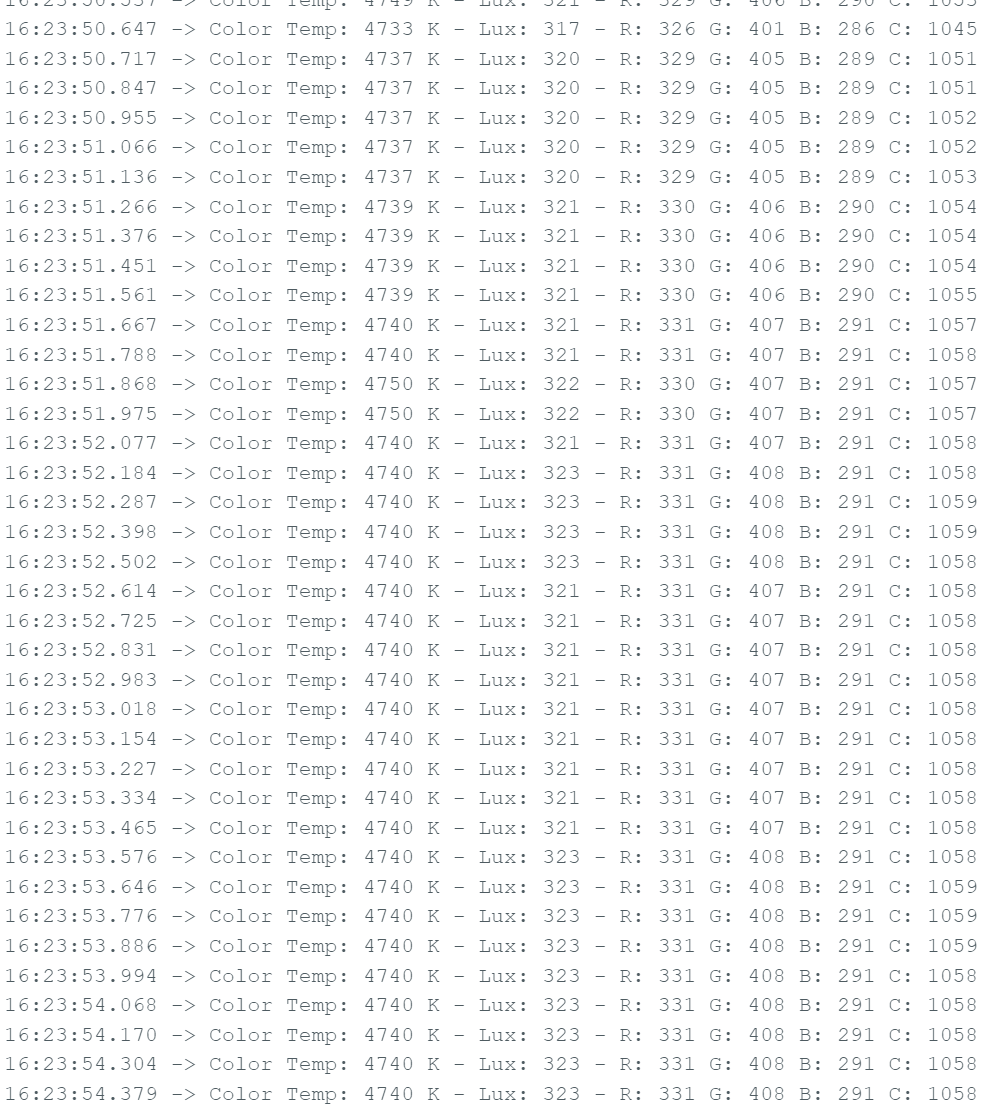
\includegraphics[width=\linewidth]{img/sensortest/MD_Linie_101ms.png}
        \caption{Messdaten Linie}
        \label{fig:MD_Farbsens}
    \end{subfigure}
    % Oben rechts
    \begin{subfigure}{0.35\textwidth}
        \centering
        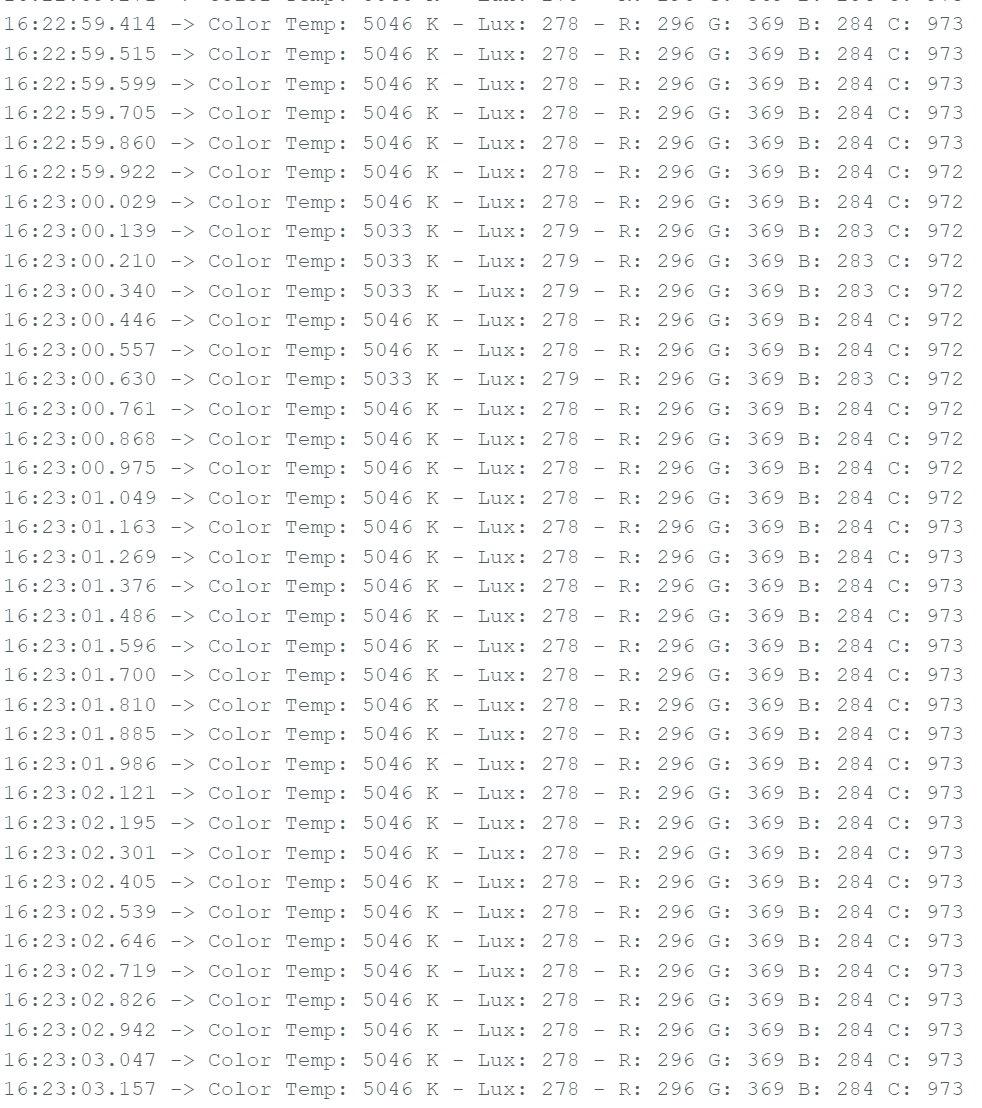
\includegraphics[width=\linewidth]{img/sensortest/MD_WeisserPunkt_101ms.png}
        \caption{Messdaten weisser Punkt}
        \label{fig:MDFarbsensorWeisserPunkt}
    \end{subfigure}
    
    % Abstand zwischen den Reihen
    \vspace{0.5cm}

    % Unten links
    \begin{subfigure}{0.35\textwidth}
        \centering
        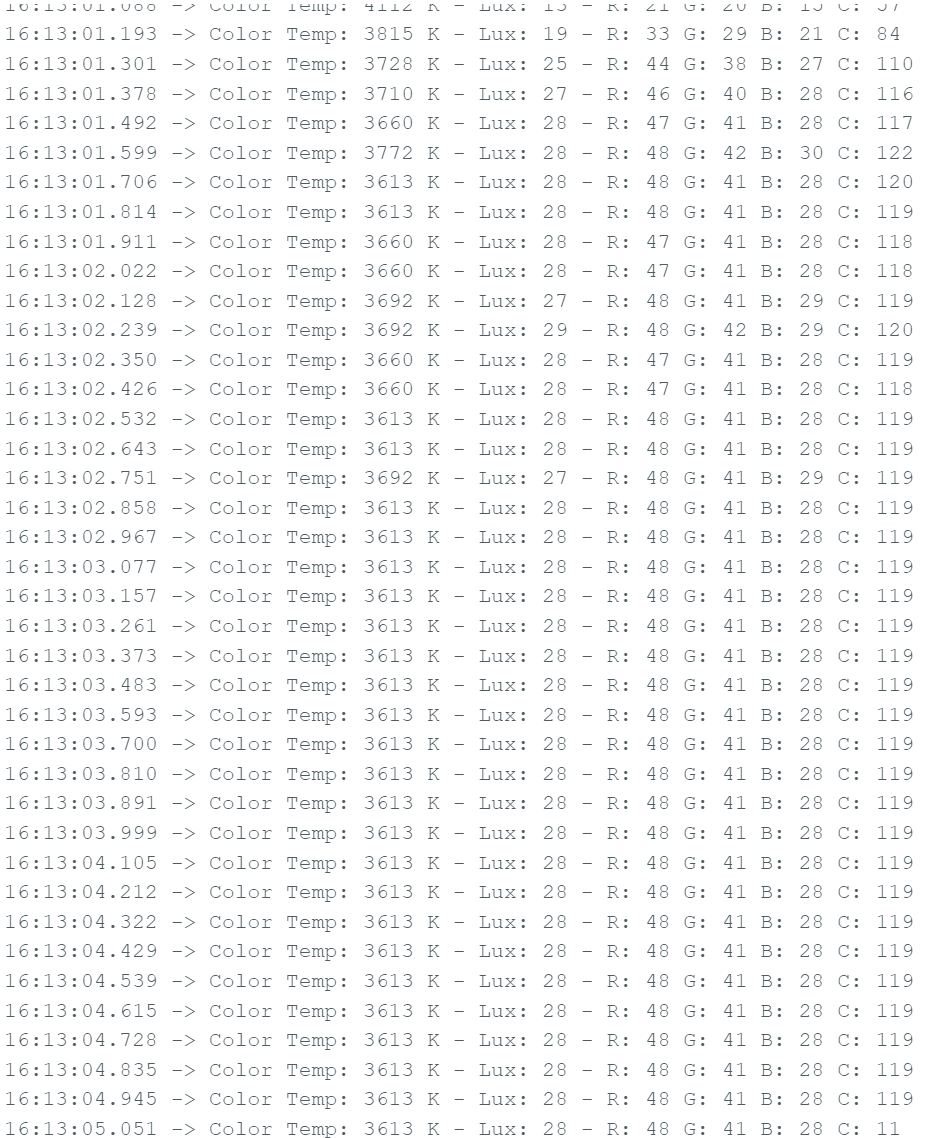
\includegraphics[width=\linewidth]{img/sensortest/MD_RotePlatte_101ms.png}
        \caption{Messdaten rote Platte}
        \label{fig:MDFarbsensorPlatte}
    \end{subfigure}
    % Unten rechts
    \begin{subfigure}{0.35\textwidth}
        \centering
        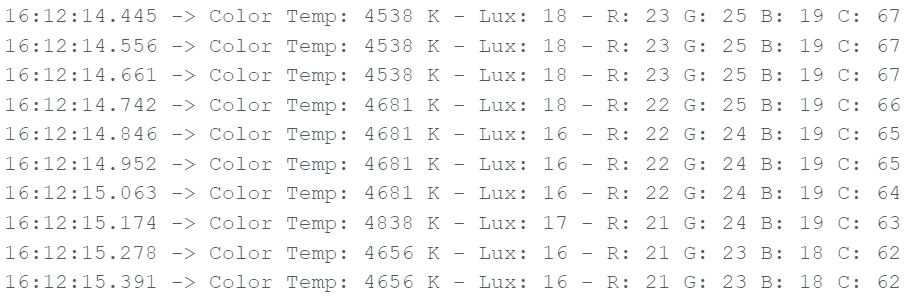
\includegraphics[width=\linewidth]{img/sensortest/MD_Fuge_101ms.png}
        \caption{Messdaten Fuge}
        \label{fig:MDFarbsensorFuge}
    \end{subfigure}

    \caption{Messdaten Farbsensor}
    \label{fig:Testanordnungen}
\end{figure}

Aus den Messdaten geht hervor, dass der Lux-Wert den grössten Unterschied zwischen den getesteten Oberflächen aufweist. Auf der Linie beträgt der Lux-Wert 320, während er auf dem weissen Punkt bei 280 liegt, wodurch die Linie vom Punkt unterschieden werden kann. Die rote Platte hat einen Lux-Wert von 28 und die Fuge einen Wert von 14, die deutlich von den 320 der Linie abweichen. Daher ist es mit dem Farbsensor möglich, die Linie zu erkennen.

Ein erheblicher Nachteil ergibt sich jedoch durch die Belichtungszeit. Da alle 101 ms ein neuer Messwert geliefert wird, bedeutet dies, dass bei einer maximalen Geschwindigkeit von 20 cm/s alle 2 cm ein neuer Wert erfasst werden kann. Dies könnte dazu führen, dass der Farbsensor die Linie verliert oder von ihr abweicht, bevor er einen neuen Messwert einlesen kann. Aus diesem Grund scheidet der Farbsensor aus.


\subsubsection{Infrarot-Linien-Array}
Eine alternative Methode zur Linienerkennung besteht in der Verwendung einer Infrarot- (IR) LED und eines IR-Fototransistors. Auf einer hellen Oberfläche werden die IR-Strahlen stärker reflektiert, wodurch der Fototransistor besser leitet. Dies führt zu niedrigeren Spannungen über dem Fototransistor auf reflektierenden Oberflächen. Mithilfe eines AD-Wandlers (Analog-Digital-Wandler) können diese Spannungen von einem Mikrocontroller ausgelesen werden.

Da viele Mikrocontroller nur eine begrenzte Anzahl an AD-Wandlern besitzen, gibt es eine alternative Lösung mithilfe eines Kondensators. Zunächst wird der Kondensator entladen, indem der entsprechende Pin (im Schema als ''Osci" bezeichnet) auf 3,3 V gesetzt wird (siehe Abbildung \ref{fig:IR_Schema}). Anschliessend wird der Pin auf Input-Capture umgestellt. Der Kondensator lädt sich daraufhin mit dem Strom des Fototransistors auf. Der Mikrocontroller misst die Zeit, bis die Spannung am Eingangs-Pin auf GND gefallen ist.

Da der Strom des Fototransistors bei stärker reflektierenden Oberflächen zunimmt, lässt sich auf diese Weise die Linie erkennen. Um die Erkennung noch zuverlässiger zu gestalten, können mehrere Fototransistoren und IR-Leuchtdioden nebeneinander angeordnet werden. Diese parallele Anordnung ermöglicht es, die Position der Linie präzise zu erfassen, selbst wenn sie sich verschiebt.


\begin{figure}[H] % 'h' steht für here, was bedeutet, dass das Bild möglichst an dieser Stelle eingefügt wird
    \centering
    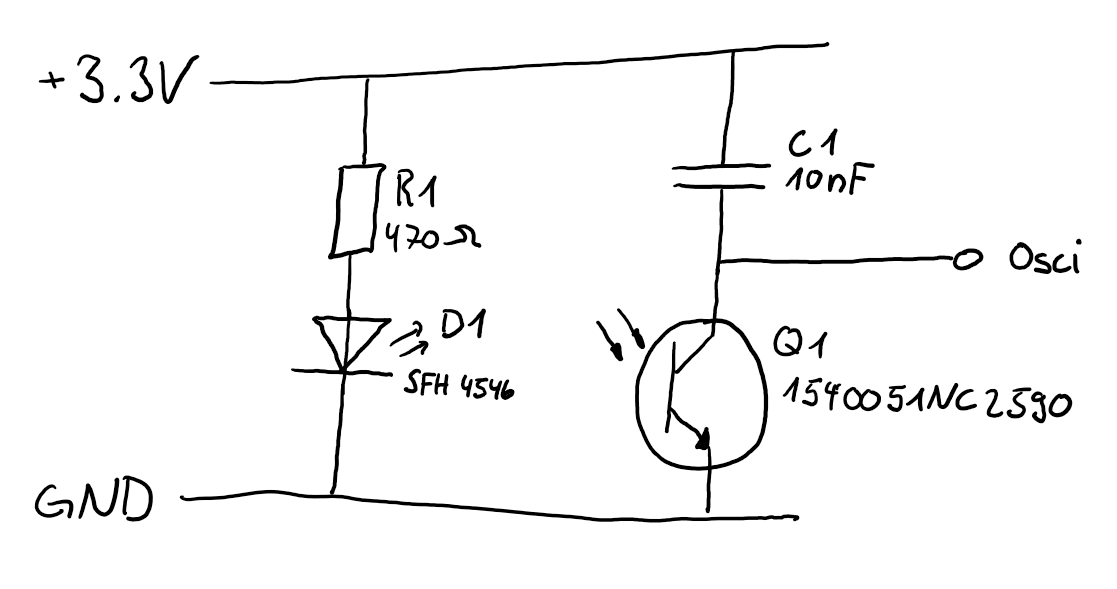
\includegraphics[width=0.7\textwidth]{img/sensortest/IR_Schema.png} % Bildname und Breite der Grafik angeben
    \caption{IR Testschema Aufbau}
    \label{fig:IR_Schema} % Label für die Referenzierung der Abbildung
\end{figure}

Mit dem Oszilloskop wurden drei Messungen auf verschiedenen Oberflächen durchgeführt. Zunächst wurde das weisse Klebeband gemessen (siehe Abbildung \ref{fig:IR_Klebeband}). Dabei zeigte sich eine steile Spannungsänderung von 3,3 V auf GND. Die Dauer des Spannungswechsels beträgt, wie unten links bei
ΔX zu sehen ist, 160 µs.

Als Nächstes wurde eine schwarze Oberfläche getestet. Hier ergab sich ein ΔX von nahezu 2 ms (siehe Abbildung \ref{fig:IR_Schwarz}). Die Differenz zwischen diesen beiden Tests beträgt somit 1840 µs, was ausreicht, um die Linie zuverlässig zu erkennen. Diese Differenz könnte weiter erhöht werden, indem ein Kondensator mit grösserer Kapazität verwendet wird.

In der dritten Messung wurde der Sensor ohne Untergrund, also nur auf die Luft gerichtet, getestet. Diese Messung ergab ein ΔX von 1,71 ms (siehe Abbildung \ref{fig:IR_Luft}). Dies bedeutet, dass der Sensor ohne einen Untergrund eine schwarze Oberfläche erkennt.

\begin{figure}[htbp]
    \raggedright
    % Erstes Bild
    \begin{subfigure}[b]{0.3\textwidth}
        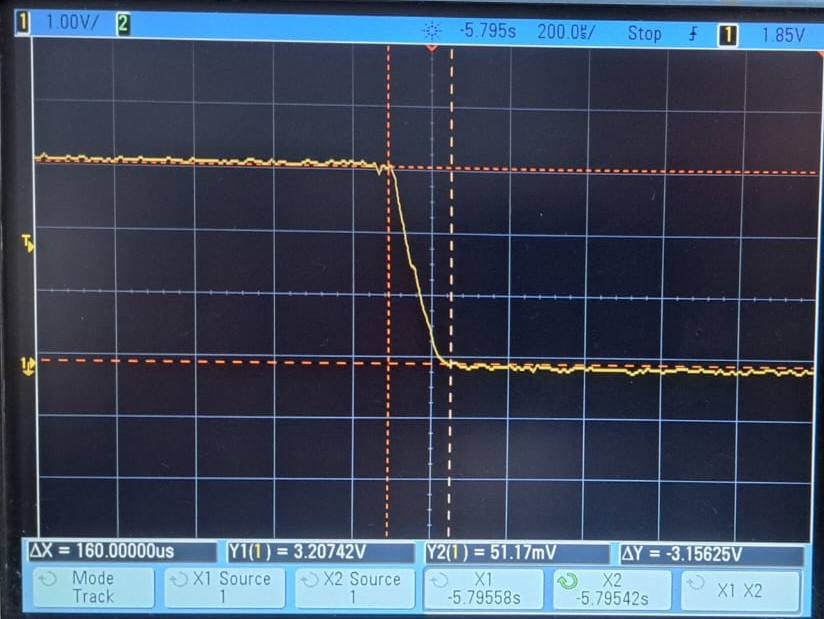
\includegraphics[height=4cm]{img/sensortest/IR_Klebeband.jpg}
        \caption{Messung Klebeband}
        \label{fig:IR_Klebeband}
    \end{subfigure}
    \hspace{0.2cm}  % Horizontaler Abstand
    % Zweites Bild
    \begin{subfigure}[b]{0.3\textwidth}
        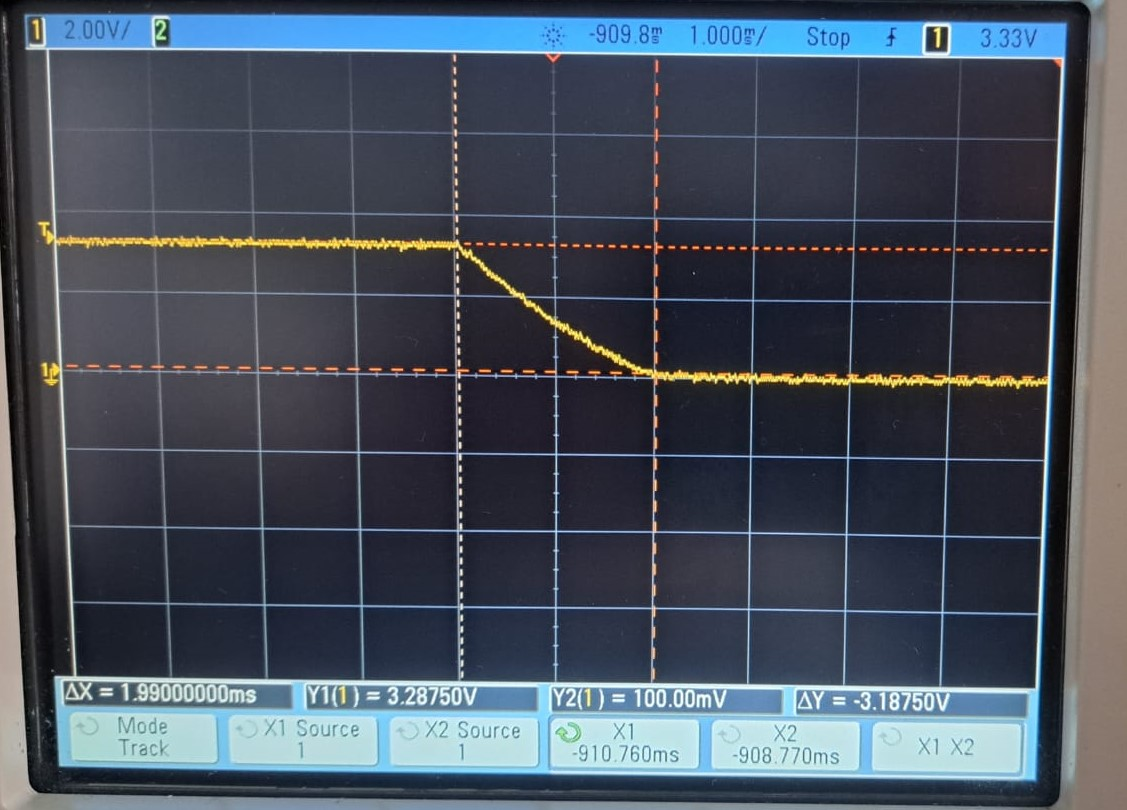
\includegraphics[height=4cm]{img/sensortest/IR_Schwarz.jpg}
        \caption{Messung Schwarz}
        \label{fig:IR_Schwarz}
    \end{subfigure}
    \hspace{0.5cm}  % Horizontaler Abstand
    % Drittes Bild
    \begin{subfigure}[b]{0.3\textwidth}
        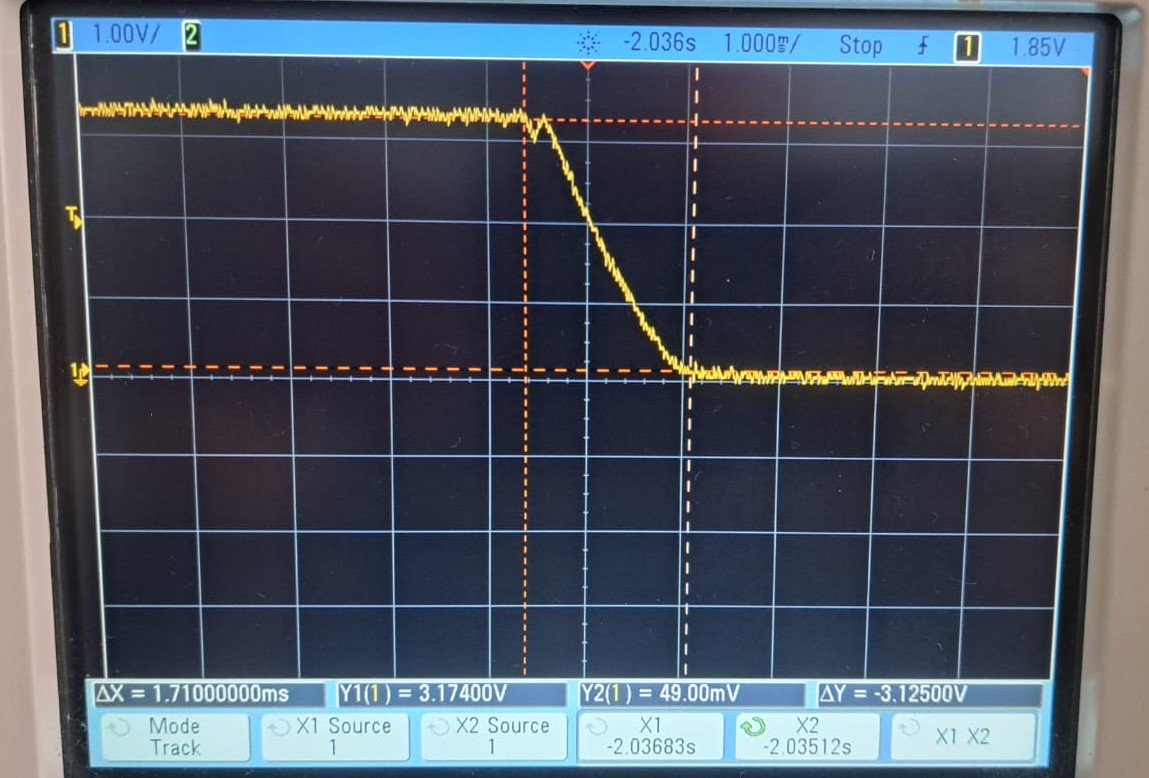
\includegraphics[height=4cm]{img/sensortest/IR_Luft.jpg}
        \caption{Messung Luft}
        \label{fig:IR_Luft}
    \end{subfigure}
    \caption{IR-Messungen Oszilloskop}
    \label{fig:IR_Messungen}
\end{figure}

Aufgrund dieser Ergebnisse wird die Linienerkennung mit Fototransistoren bevorzugt. Mit einem Fototransistor-Array, das mindestens 7 cm breit ist, kann auch der weisse Punkt zuverlässig erkannt werden. Denn auf der Linie wird niemals jeder Fototransistor die Linie gleichzeitig erfassen. Auf dem Punkt hingegen melden alle Fototransistoren die Erkennung der Linie, was darauf hinweist, dass es sich um den Punkt handelt.



\end{document}